\documentclass[11pt,a4paper]{jarticle}
\usepackage[dvips]{graphicx}
\usepackage{here}

\title{{触入班進捗報告\\実験計画}}
\date{2014年6月3日(火)}
\author{小森谷 大介、川畑 裕也、深津 佳智}

\begin{document}

\maketitle

%1
\section{概要}
今年度、触入班では、スマートフォンの表面(タッチパネル面)もしくは裏面に突起を付ける発展案を考えた。
この突起により、ユーザがアイズフリーにおいてタッチ入力する際の手がかりになると考えられる。
実験では、突起がタッチ精度に及ぼす影響を検証する。

本進捗資料では、実験計画、及び、突起の位置について検討したものを報告する。

%2
\section{実験計画}
以下の2種類の実験条件を設定し、被験者にアイズフリーにおいてタッチパネル上のターゲットをタッチしてもらう実験を行おうと考えている。
\begin{itemize}
  \item 突起条件:突起無し条件、表面突起A条件、表面突起B条件、表面突起C地点、背面突起A条件、背面突起B条件、背面突起C条件
  \item 分割条件:3~$\times$~3分割条件、4~$\times$~4分割条件、5~$\times$~5分割条件
\end{itemize}

昨年度の実験と今回の実験計画の相違点は、ケース条件であったところを突起条件に変え、表面もしくは背面の1点のみに突起を付けて実験を行う点である。
また、表面突起A条件と背面突起A条件、表面突起B条件と背面突起B条件、表面突起C条件と背面突起C条件の突起位置を、それぞれ、平面図において同じ位置に対応させることを考えている。
これにより、表面に突起を付けた際のタッチ精度と裏面に突起を付けた際のタッチ精度を比較することができると考えられる。

また、昨年度の実験においては開始点タッチ条件と終了点タッチ条件が存在したが、今年度の実験においては終了点タッチ条件のみとした。
この理由は、終了点タッチ条件では、表面(もしくは背面)に指を付けた状態で、表面(もしくは裏面)の突起を手さぐりで見つけ、タッチの手がかりとしやすくなると考えられる、また、実験のタスク数を増やし過ぎないためである。
なお、昨年度の実験では、開始点タッチ条件と終了点タッチ条件のタッチ精度に有意差は見られなかった。

%3
\section{突起位置の候補}
突起の位置の候補として図\ref{fig:iti}に示す6点を考えた。
\begin{figure}[H]
  \begin{center}
  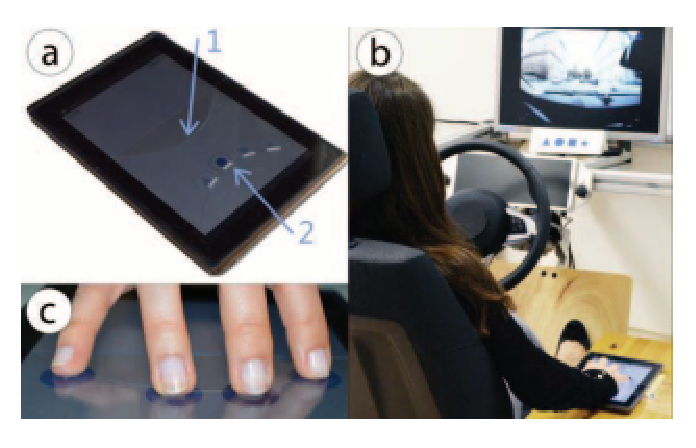
\includegraphics[width=8cm]{fig/figure1.eps}
  \caption{突起の位置候補}
  \label{fig:iti}
  \end{center}
\end{figure}

\begin{enumerate}
 \item[1.中央]\mbox{}\\
	中央の位置を把握しやすくなると考えられる
 \item[2.左上]\mbox{}\\ 
	片手把持の時、ターゲットまで距離が遠く、昨年度の実験においてはタッチ精度が最も低かった。
 \item[3.右下]\mbox{}\\
  昨年度の実験においては、タッチ精度が最も高かった。
	一方で、指が長い人にとっては、片手把持の時、親指を極端に曲げなければならずタッチしにくい領域であるとも考えられる。
 \item[4.右上]\mbox{}\\
	片手把持をした際、容易に親指を用いてタッチすることが可能な位置である。
 \item[5.左下]\mbox{}\\
	片手把持をした際、容易に親指を用いてタッチすることが可能な位置である。
 \item[6.左上端]\mbox{}\\
	片手把持をした際、もっとも遠くタッチしにくい領域である。
\end{enumerate}

%4
\section{突起位置の検討}
突起は中央点の他に左上、右下について作成することを考えている。
左上、右下の突起を作成する位置について考察を行った。

実験では、3~$\times$~3、4~$\times$~4、5~$\times$~5の3つの分割条件においてタッチ操作を行う。
そのため、これらの3条件において手がかりとしやすい位置に配置しなければならない。
3つの条件の分割線をそれぞれ、図\ref{fig:fig1}、\ref{fig:fig2}、\ref{fig:fig3}に示す。
また、3つの条件をすべて重ねた図\ref{fig:fig4}を以下に示す。

\begin{figure}[H]
  \begin{center}
  \includegraphics[width=4cm]{fig/photo1.eps}
  \caption{3×3}
  \label{fig:fig1}
  \end{center}
\end{figure}

\begin{figure}[H]
  \begin{center}
  \includegraphics[width=4cm]{fig/photo2.eps}
  \caption{4×4}
  \label{fig:fig2}
  \end{center}
\end{figure}

\begin{figure}[H]
  \begin{center}
  \includegraphics[width=4cm]{fig/photo3.eps}
  \caption{5×5}
  \label{fig:fig3}
  \end{center}
\end{figure}

\begin{figure}[H]
  \begin{center}
  \includegraphics[width=4cm]{fig/photo4.eps}
  \caption{図\ref{fig:fig1}から図\ref{fig:fig3}までを重ねた}
  \label{fig:fig4}
  \end{center}
\end{figure}

図\ref{fig:fig4}からわかるように3つの条件において重なる点は存在しない。そこで、3条件のそれぞれの交点においてもっとも点が密集している点に突起を配置すると良いのではないかと考えた。

3条件それぞれの交点において他の2条件の交点との距離を評価した。
評価としては3~$\times$~3と4~$\times$~4、3~$\times$~3と4~$\times$~4、4~$\times$~4と5~$\times$~5の3つの組み合わせに置いてすべての交点同士の距離を計算することとした。
これにより3条件すべてにおいてもっともホームポジションとして使いやすい点を計算出来るのではないかと考えた。

この評価の結果、図\ref{fig:fig5}に示す3点が3条件において最も接近している3点であることがわかった。
よってこの3点を突起をつける点として選ぶことが妥当であると考えた。
特に4~$\times$~4の点(図\ref{fig:fig5}示した3点の中央)は3~$\times$~3(図\ref{fig:fig5}示した3点の右下)と5~$\times$~5図\ref{fig:fig5}示した3点の左上)の間にあるため評価実験における基準として使用できるのではないかと考えた。

\begin{figure}[H]
  \begin{center}
  \includegraphics[width=4cm]{fig/photo5.eps}
  \caption{3条件で最も点において接近している3点}
  \label{fig:fig5}
  \end{center}
\end{figure}

%5
\section{今後の予定}
7月にHCI研究会もしくはHISに投稿した後に、HCIIに出せるのが理想的なルート
\begin{itemize}
  \item 6月
  \begin{itemize}
    \item 実験
  \end{itemize}
  \item 7月
  \begin{itemize}
    \item HCI研究会(日程未定)
  \end{itemize}
  \item 8月
  \begin{itemize}
    \item 31日 HCIIアブスト締切(去年の日程)
  \end{itemize}
\end{itemize}
\bibliographystyle{jalpha}
\bibliography{shokunyu}
\end{document}
